\documentclass{aitthesis}
\usepackage{amsmath,amssymb}
\usepackage{multirow}
\usepackage{graphicx}
\usepackage{subfig}
\usepackage{booktabs}
\usepackage{comment}

\bibliographystyle{apacite}

\begin{document}

\pagenumbering{roman}
\addtocontents{toc}{~\hfill\textbf{Page}\par} %This adds the word Page on top of the table of content

\addcontentsline{toc}{chapter}{\bf TITLE PAGE}
\begin{comment}
\setcounter{page}{1}
\thispagestyle{empty} 

\phantomsection
\begin{center}
    \large{\bf ALIGN-VQA: ALIGNMENT-GUIDED RESIDUAL MODELING
    	FOR LONGITUDINAL MEDICAL VISUAL QUESTION ANSWERING}

\vskip 2em
by
\vskip 2em
Kaung Sithu
\vskip 2em
A Thesis Submitted in Partial Fulfillment of the
Requirements for the\\ Degree of Master of Engineering in
Data Science and Artificial Intelligence

%	\vskip 5em
\vskip 1em
{
  \begin{center}
    \begin{tabular}{rl}
      \\[-1em]
      Examination Committee: & Dr.\ Chaklam Silpasuwanchai (Chairperson) \\
                             & Prof.\ Mongkol Ekpanyapong (Member) \\
                             & Dr. Chantri Polprasert (Member) \\
	    \\
	    \\
      Nationality:     & Myanmar \\
      Previous Degree: & Bachelor of Engineering in Information Technology \\
                       & West Yangon Technological University \\
                       & Myanmar \\
      \\
      Scholarship Donor: & AIT Scholarships\\
      \\
    \end{tabular}
  \end{center}

  \vskip 1em
}
\vfill
\end{center}
\begin{center}
  Asian Institute of Technology\\ School of Engineering
                  and Technology\\ Thailand\\ May 2026
\end{center}
\vfill
\end{comment}

\setcounter{page}{1}
\thispagestyle{empty} 

\phantomsection
\begin{center}
	\large\textbf{ALIGNMENT-GUIDED RESIDUAL MODELING FOR LONGITUDINAL MEDICAL VISUAL QUESTION ANSWERING}
	
	\vspace{2em}
	by\\
	\vspace{2em}
	Kaung Sithu
	\vspace{2em}
	
	A Thesis Submitted in Partial Fulfillment of the\\
	Requirements for the Degree of Master of Engineering in\\
	Data Science and Artificial Intelligence
	
	\vspace{2em}
	
	\begin{tabular}{rl}
		\\[-1em]
		Examination Committee: & Dr.\ Chaklam Silpasuwanchai (Chairperson) \\
		& Prof.\ Mongkol Ekpanyapong (Member) \\
		& Dr.\ Chantri Polprasert (Member) \\
		\\
		Nationality:     & Myanmar \\
		Previous Degree: & Bachelor of Engineering in Information Technology\\
		& West Yangon Technological University, Myanmar \\
		\\
		Scholarship Donor: & AIT Scholarships\\
		\\
	\end{tabular}
	
	% \vfill acts like a spring, pushing the text below it to the very bottom of the page
	\vfill 
	
	Asian Institute of Technology\\ 
	Faculty of Advanced Science and Technology\\ 
	Thailand\\ 
	May 2026
\end{center}
\clearpage % Ensures the next content starts cleanly on page 2
\include{declaration}
\phantomsection
\addcontentsline{toc}{chapter}{\bf ACKNOWLEDGEMENTS}
\begin{center}
    \large{\bf ACKNOWLEDGEMENTS}
\end{center}

I would like to express my sincere gratitude to all those who have supported me throughout this Master's thesis.

First, I wish to acknowledge the partial financial support provided by AIT scholarships. This support was instrumental in allowing me to dedicate my focus to this research.

I am deeply indebted to my supervisor, Dr. Chaklam Silpasuwanchai, assistant professor, for their invaluable guidance, insightful feedback, and unwavering support from the beginning to the end of this project. Their expertise was essential to the direction and success of this work.

I would also like to extend a special thanks to Ms. Deepali Mishra, whose weekly meetings, practical advice, and consistent encouragement were a source of great help and motivation.
\phantomsection
\addcontentsline{toc}{chapter}{\bf ABSTRACT}

\begin{center}
    \large{\bf ABSTRACT}
\end{center}

Longitudinal image comparison is fundamental to radiological decision-making, requiring clinicians to assess the temporal evolution of findings across visits. Medical Difference Visual Question Answering (Diff-VQA) formalizes this process, however, the current methods for Diff-VQA often rely on direct feature subtraction or simple fusion. These strategies assume inherent spatial correspondence, a premise frequently violated by stochastic acquisition variability and non-rigid anatomical deformations in clinical practice. The author proposes ALIGN-VQA, a novel alignment-guided residual modeling architecture for robust temporal reasoning. Thisg approach introduces three key innovations: (i) Cross-Image Difference Attention (CIDA): Aligns prior-visit features to the current scan via semantic reconstruction, ensuring misalignment-tolerant comparison, (ii) Learnable Residual Gating: Captures precise deviations between aligned historical and current representations to extract evolution-aware features, (iii) Question-Guided Difference Tokenizer (QDT): Selectively pools question-relevant temporal changes for targeted reasoning. Evaluation on the Medical-Diff-VQA benchmark, ALIGN-VQA shows comparable or better performance compared to state-of-the-art methods, with notable improvements in complex reasoning categories. Further, the proposed model ALIGN-VQA is a lightweight architecture making it amenable for edge deployments.

\include{contents}
\include{loft}

\pagestyle{plain}
\pagenumbering{arabic}

\chapter{INTRODUCTION} 

\section{Background of the Study}
The automated interpretation of longitudinal radiological images, a cornerstone of clinical practice, has recently been formalized under the task of Difference Visual Question Answering (DiffVQA). The release of \cite{medical-diff-vqa} was a pivotal moment, enabling the development of models to answer nuanced questions about temporal changes in patient scans. The subsequent evolution of state-of-the-art models has revealed a consistent, yet resource-intensive, paradigm.

Initial architectural innovations, such as the graph-based representations in \cite{ekaid} and the dedicated residual encoder in \cite{real}, established methods for processing paired image features. However, these models operate on dense visual feature maps, a computationally expensive approach. Recognizing the need for stronger representations, \cite{plural} demonstrated that extensive pre-training on large-scale natural and medical corpora significantly boosts performance, but at the cost of being highly data-hungry and dependent on external reports. More recently, retrieval-augmented models like \cite{regiomix} and powerful backbones like the Swin Transformer in the \cite{encoder-decoder} have pushed performance further. While these models are highly effective, they represent a "brute-force" methodology: they rely on massive model scale, computationally expensive database searches, or the processing of thousands of visual tokens from the entire image to implicitly learn the difference signal.

\section{Statement of the Problem}
The dominant paradigm in Difference VQA is fundamentally inefficient and lacks explicit clinical reasoning. Current models are computationally expensive, requiring the processing of dense visual information from two full images, even when the question pertains to a small, localized change. This brute-force approach is not only wasteful but also fails to explicitly model the directionality of clinical findings, making it difficult to distinguish between concepts like missing or new abnormalities. Furthermore, this reliance on large, complex models without learning gating mechanism makes them prone to capturing non-pathological changes that are not relevant, a critical failure for any clinical support tool. The field lacks a model that is computationally efficient, explicitly models the direction of change, and filters out non-pathological visual noise and static anatomy

\section{Research Questions}
Following the problem, There are three research questions:
\begin{enumerate}
    \item Can longitudinal, difference-focused questions be accurately answered using only a handful of question-guided difference tokens, instead of processing all image patches?
    \item Does the cross image difference attention help the model distinguish the direction of change such as missing or new abnormalities?
    \item Does the application of a learnable residual gating mechanism impact the model's ability to capture precise pathologies?
\end{enumerate}

\section{Hypotheses}
There are three hypotheses to answer the research question:
\begin{enumerate}
    \item A small set of sparse, question-guided difference tokens is sufficient to achieve state-of-the-art performance, leading to a dramatic increase in computational efficiency.
    \item Aligning reference image to current image yields more accurate representation of disease evolution than direct substraction.
    \item Applying a learnable gating mechanism to residual features effectively filters out non-pathological noise, resulting in higher diagnostic accuracy.
\end{enumerate}

\section{Objectives of the Study}
The main objective is to design and develop lightweight, difference aware medical VQA system that can provide faithful visual evidence to support its answer while being compute efficient and not requiring retrieval databases, radiology reports or expert annotations. The sub-objectives are:

\begin{enumerate}
    \item To validate the effectiveness of a Question-Guided Diffference Tokenizer (QDT) at distilling visual information into a sparse set of tokens.
    \item To evaluate the impact of an integrated Cross Image Difference Attention (CIDA) on the model's ability to reason about the direction of clinical change.
    \item To quantify the impact of the learnable residual gating mechanism in isolating precise pathological deviations and extracting evolution-aware features.
\end{enumerate}

\section{Methodology}
This work introduces ALIGN-VQA, a novel, lightweight architecture that shifts from a brute-force comparison to an alignment-guided residual modeling paradigm. The methodology is centered on three key innovations designed to handle the stochastic acquisition variability and non-rigid anatomical deformations inherent in longitudinal imaging. First, to overcome the limitations of spatial misalignment between scans, the CIDA module semantically aligns prior-visit features to the current scan via cross-attention before computing differences. This aligned representation is then passed through a Learnable Residual Gating mechanism, which adaptively suppresses acquisition noise to extract precise, evolution-aware residual features. Second, the QDT module utilizes domain-aware text embeddings from ClinicalBERT to evaluate the relevance of these visual deviations by applying cross-attention to selectively pool only the Top-K most clinically salient temporal changes. The vision components learn contextual coherence via a self-supervised Masked Residual Modeling (MRM) task, while an auxiliary multi-label classification head explicitly ground the visual features in 14 thoracic pathologies. 


\section{Scope}
In scope:
\begin{itemize}
    \item The thesis will exclusively use the public Medical-Diff-VQA dataset, focusing on all question categories for all experiments.
    \item The core of the work is the design, implementation, and evaluation of our novel, lightweight VQA architecture and its specific modules (CIDA, QDT, CFA-Reg, MRM).
    \item Evaluation will consist of targeted ablation studies and a direct benchmark against a comprehensive suite of SOTA models (EKAID, ReAl, PLURAL, RegioMix, VED).
\end{itemize}

Out of scope:
\begin{itemize}
	\item This work will not involve the collection of new clinical data or the execution of clinical trials with human radiologists.
	\item This thesis will not develop a new, general-purpose medical VQA system.
\end{itemize}


\section{Expected Key Findings}
\begin{itemize}
	\item The proposed, ALIGN-VQA, model is expected to achieve performance comparable or superior to current state-of-the-art models with a fraction of the computational cost, demonstrating the viability of an efficiency-focused paradigm.
	
	\item The integration of CIDA module will be shown to provide a significant accuracy boost by explicitly handling spatial misalignments and suppressing stochastic acquisition noise, particularly excelling in complex comparative reasoning categories.
	
	\item The learnable gating mechanism will be proven to isolate true pathological deviations from visual noise and static anatomy
\end{itemize}

\section{Contribution}
\begin{itemize}
	\item This thesis introduces ALIGN-VQA, a novel, lightweight paradigm for DiffVQA centered on efficiency, explicit reasoning, and robustness, shifting the field away from the dominant brute-force, resource-intensive methodologies.
	\item Three key architectural innovations are developed, CIDA module for misalignment-tolerant semantic reconstruction, learnable residual gating for isolating true evolution-aware features, and a QDT module that selectively pools clinically salient tokens to prevent signal dilution and maximize computational efficiency.
	\item A comprehensive multi-stage training strategy that incorporates self-supervised MRM, auxiliary disease classification, and counterfactual learning—is introduced. This yields a state-of-the-art framework that is robust, computationally accessible, and self-contained, removing the reliance on massive external radiology report corpora for pre-training.
\end{itemize}
\setlength{\footskip}{8mm}

\chapter{RELATED WORK}
This chapter critically examines the existing body of literature to contextualize ALIGN-VQA architecture and the research questions driving this thesis. Longitudinal medical imaging is a cornerstone of radiological diagnosis, requiring clinicians to meticulously track disease progression or stability over time. In response, Difference-aware Medical VQA (Diff-VQA) has emerged as a specialized domain designed to analyze paired longitudinal scans and answer complex clinical queries regarding their differences. However, despite rapid advancements in generative vision-language models, current Diff-VQA architectures remain constrained by several critical methodological bottlenecks.

\section{Difference Modeling and the Alignment Problem in Longitudinal VQA}
Early approaches to this problem, such as \cite{ekaid}, attempt to structure the comparison by representing anatomical regions as nodes in a multi-relationship graph. By extracting features from identical anatomical bounding boxes across two temporal scans, it aims to evaluate disease progression within specific lung regions. While this explicitly incorporates spatial and semantic medical priors, its reliance on a pre-trained \cite{faster-rcnn} to detect bounding boxes leaves the model vulnerable; inaccurate feature extraction directly results in incorrect comparative predictions. Furthermore, this strict graph structure struggles to adapt to non-rigid anatomical deformations or novel structural changes not predefined in the knowledge graph.

More recent models, such as \cite{real}, compute temporal differences by directly subtracting the reference image from the main image to produce a residual input. This residual is processed through an independent encoder, guided by a consistency loss to enforce focus on disparate regions. However, direct subtraction strategies implicitly assume perfect spatial correspondence between the two scans. In clinical practice, this assumption is frequently violated due to stochastic acquisition variability, patient movement, and postural differences between visits. When raw image subtraction is applied to misaligned scans, it generates overwhelming artifact noise rather than isolating true pathological evolution.

\section{Feature Selection and Computational Efficieny}
\cite{plural} created addresses longitudinal VQA by concatenating the flattened feature vectors of both the past and current images into a single, massive sequence. Utilizing \cite{resnet101}, it generates 576 tokens per image, resulting in a dense, highly redundant input matrix that is processed by a 6-layer Transformer encoder-decoder. While PLURAL benefits from large-scale pretraining on external datasets like \cite{mimic-cxr} and \cite{MS-COCO}, its brute-force processing of all spatial patches limits its efficiency and scalability.

Similarly, \cite{encoder-decoder} model utilizes a Swin Transformer backbone combined with an Image Differentiation Embedding (IDE) to differentiate the temporal scans. While their model utilizes a lightweight 3-layer decoder, it still fuses and processes the full visual feature maps via cross-attention to generate answers. Other paradigms, such as \cite{regiomix}, attempt to bypass heavy paired-image processing by using Retrieval-Augmented Generation (RAG) to mix-and-match retrieved region features from an external database. While innovative, it requires a continuous, computationally expensive database search for every query and struggles to reason over novel differences not present in the retrieval set.



\section{Mitigating Hallucination and Dataset Biases through Counterfactual Training}
A persistent weakness in generative medical vision-language models is their propensity to hallucinate findings or rely on spurious dataset correlations rather than true visual evidence. Generative Diff-VQA models are particularly susceptible to this, as they must predict complex sequences describing evolving pathologies.
Error analyses of current state-of-the-art models expose the clinical dangers of these hallucinations. For instance, evaluations of \cite{plural} demonstrate instances where the architecture accurately identifies regions of interest but hallucinates the severity sequence, describing an abnormality in reverse temporal order. Similarly, researchers evaluating \cite{encoder-decoder} noted a critical divergence between automated Natural Language Generation (NLG) metrics and clinical correctness.It frequently achieved near-perfect scores on metrics like \cite{bleu} and ROUGE-L, yet clinical review revealed the model was misinterpreting diagnoses—often hallucinating the resolution of anomalies that had not actually subsided, or identifying new anomalies that were not present in the scans. This confirms that standard generative training heavily biases models toward the linguistic distribution of the training reports rather than grounded visual reasoning.


\section{Hypothesis and Positioning}
Existing methods indiscriminately process background and irrelevant features, diluting the model's focus on the actual clinical question. This thesis hypothesizes that longitudinal, difference-focused questions can be accurately answered using only a handful of question-guided difference tokens. By introducing a Question-Guided Difference Tokenizer (QDT) that uses cross-attention to score and select only the Top-K most query-relevant visual residual tokens, the proposed model will explicitly filter out irrelevant changes, drastically reducing the computational load for the downstream language model while preventing the dilution of clinically salient deviations.

The limitations of direct subtraction and rigid graph mapping present a critical gap in modeling the direction and accuracy of temporal changes. This research hypothesizes that a Cross-Image Difference Attention (CIDA) module can overcome these limitations by semantically reconstructing and aligning prior-visit features to the current scan's spatial layout via cross-attention before computing residuals. This alignment-guided approach is expected to provide a highly robust mechanism for distinguishing the true direction of change without being derailed by standard acquisition misalignments.

Standard cross-entropy optimization allows models to memorize language priors, leading to hallucinations on unchanged or subtly different image pairs. This research hypothesizes that counterfactual training, specifically combining hierarchical Kullback-Leibler (KL) divergence with Noise Contrastive Estimation (NCE), will force the model to explicitly disentangle true causal temporal evolution from nuisance visual patterns and dataset biases. By contrasting positive longitudinal pairs against logically opposite or synthetically perturbed counterfactual samples, the model is expected to significantly reduce its false positive hallucination rate on unchanged image pairs.




\section{Comparative Analysis of Methodologies}
The following table summarizes the key limitations of the current state-of-the-art models.

\begin{table}[h!]
	\centering
	\caption{Comparative Analysis of Limitations in State-of-the-Art DiffVQA Models.}
	\label{tab:sota_limitations}
	\resizebox{\textwidth}{!}{%
		\begin{tabular}{lcccc}
			\hline
			\textbf{Model/Methodology} & \textbf{\begin{tabular}[c]{@{}c@{}}Computational\\ Inefficiency\end{tabular}} & \textbf{\begin{tabular}[c]{@{}c@{}}Spatial Misalignment Vulnerability\\ Reasoning\end{tabular}} & \textbf{\begin{tabular}[c]{@{}c@{}}High Data\\ Dependency\end{tabular}} & \textbf{\begin{tabular}[c]{@{}c@{}}Lacks Explicit\\ Robustness Training\end{tabular}} \\ \hline
			\cite{ekaid} & \checkmark & \checkmark & & \checkmark \\
			\cite{real} & \checkmark & \checkmark & & \checkmark \\
			\cite{regiomix} & \checkmark & & \checkmark & \checkmark \\
			\cite{plural} & \checkmark & \checkmark & \checkmark & \checkmark \\
			\cite{encoder-decoder} & \checkmark & \checkmark & & \checkmark \\ \hline
			\textbf{Our Proposed Model} & \textit{Addressed by QDT} & \textit{Addressed by CIDA} & \textit{Addressed by MRM} & \textit{Addressed by Counterfactual Learning} \\ \hline
		\end{tabular}%
	}
\end{table}

\begin{table}[h!]
	\centering
	\caption{Mapping of Proposed Components to Research Gaps}
	\label{tab:component_mapping_booktabs}
	\resizebox{\textwidth}{!}{%
	\begin{tabular}{lll}
		\toprule
		\textbf{Proposed Component} & \textbf{Research Gap Addressed} & \textbf{Corresponding Research Question} \\ 
		\midrule
		Question-Guided Difference & Computational inefficiency of & RQ1: Can longitudinal questions be answered using \\
		Tokenizer (QDT) & processing dense visual features. & only a handful of question-guided difference tokens? \\
		\addlinespace
		Directional Residual Stack & Vulnerability to spatial misalignments and implicit & RQ2: Does cross-image difference attention help \\
		(DRS) & assumptions of direct feature substraction & the model distinguish the direction of change? \\
		\addlinespace
		Counterfactual Regularizer & vulnerability of generative models  & RQ3: Can counterfactual training reduce \\
		(CFA-Reg) & to clinical hallucination and dataset biases & the tendency of the model to hallucinate? \\
		\bottomrule
	\end{tabular}
}
\end{table}

\setlength{\footskip}{8mm}

\chapter{METHODOLOGY}


\section{Architectureal Overview}

Longitudinal medical image comparison requires models to distinguish true pathological evolution from stochastic acquisition variability, such as patient movement or differences in posture. Conventional Difference-aware Medical VQA methods rely on direct feature subtraction, which implicitly assumes perfect spatial correspondence between scans. This thesis introduces ALIGN-VQA, an alignment-guided residual modeling architecture designed to overcome these spatial misalignment vulnerabilities.

\begin{figure}[htbp]
	\centering
	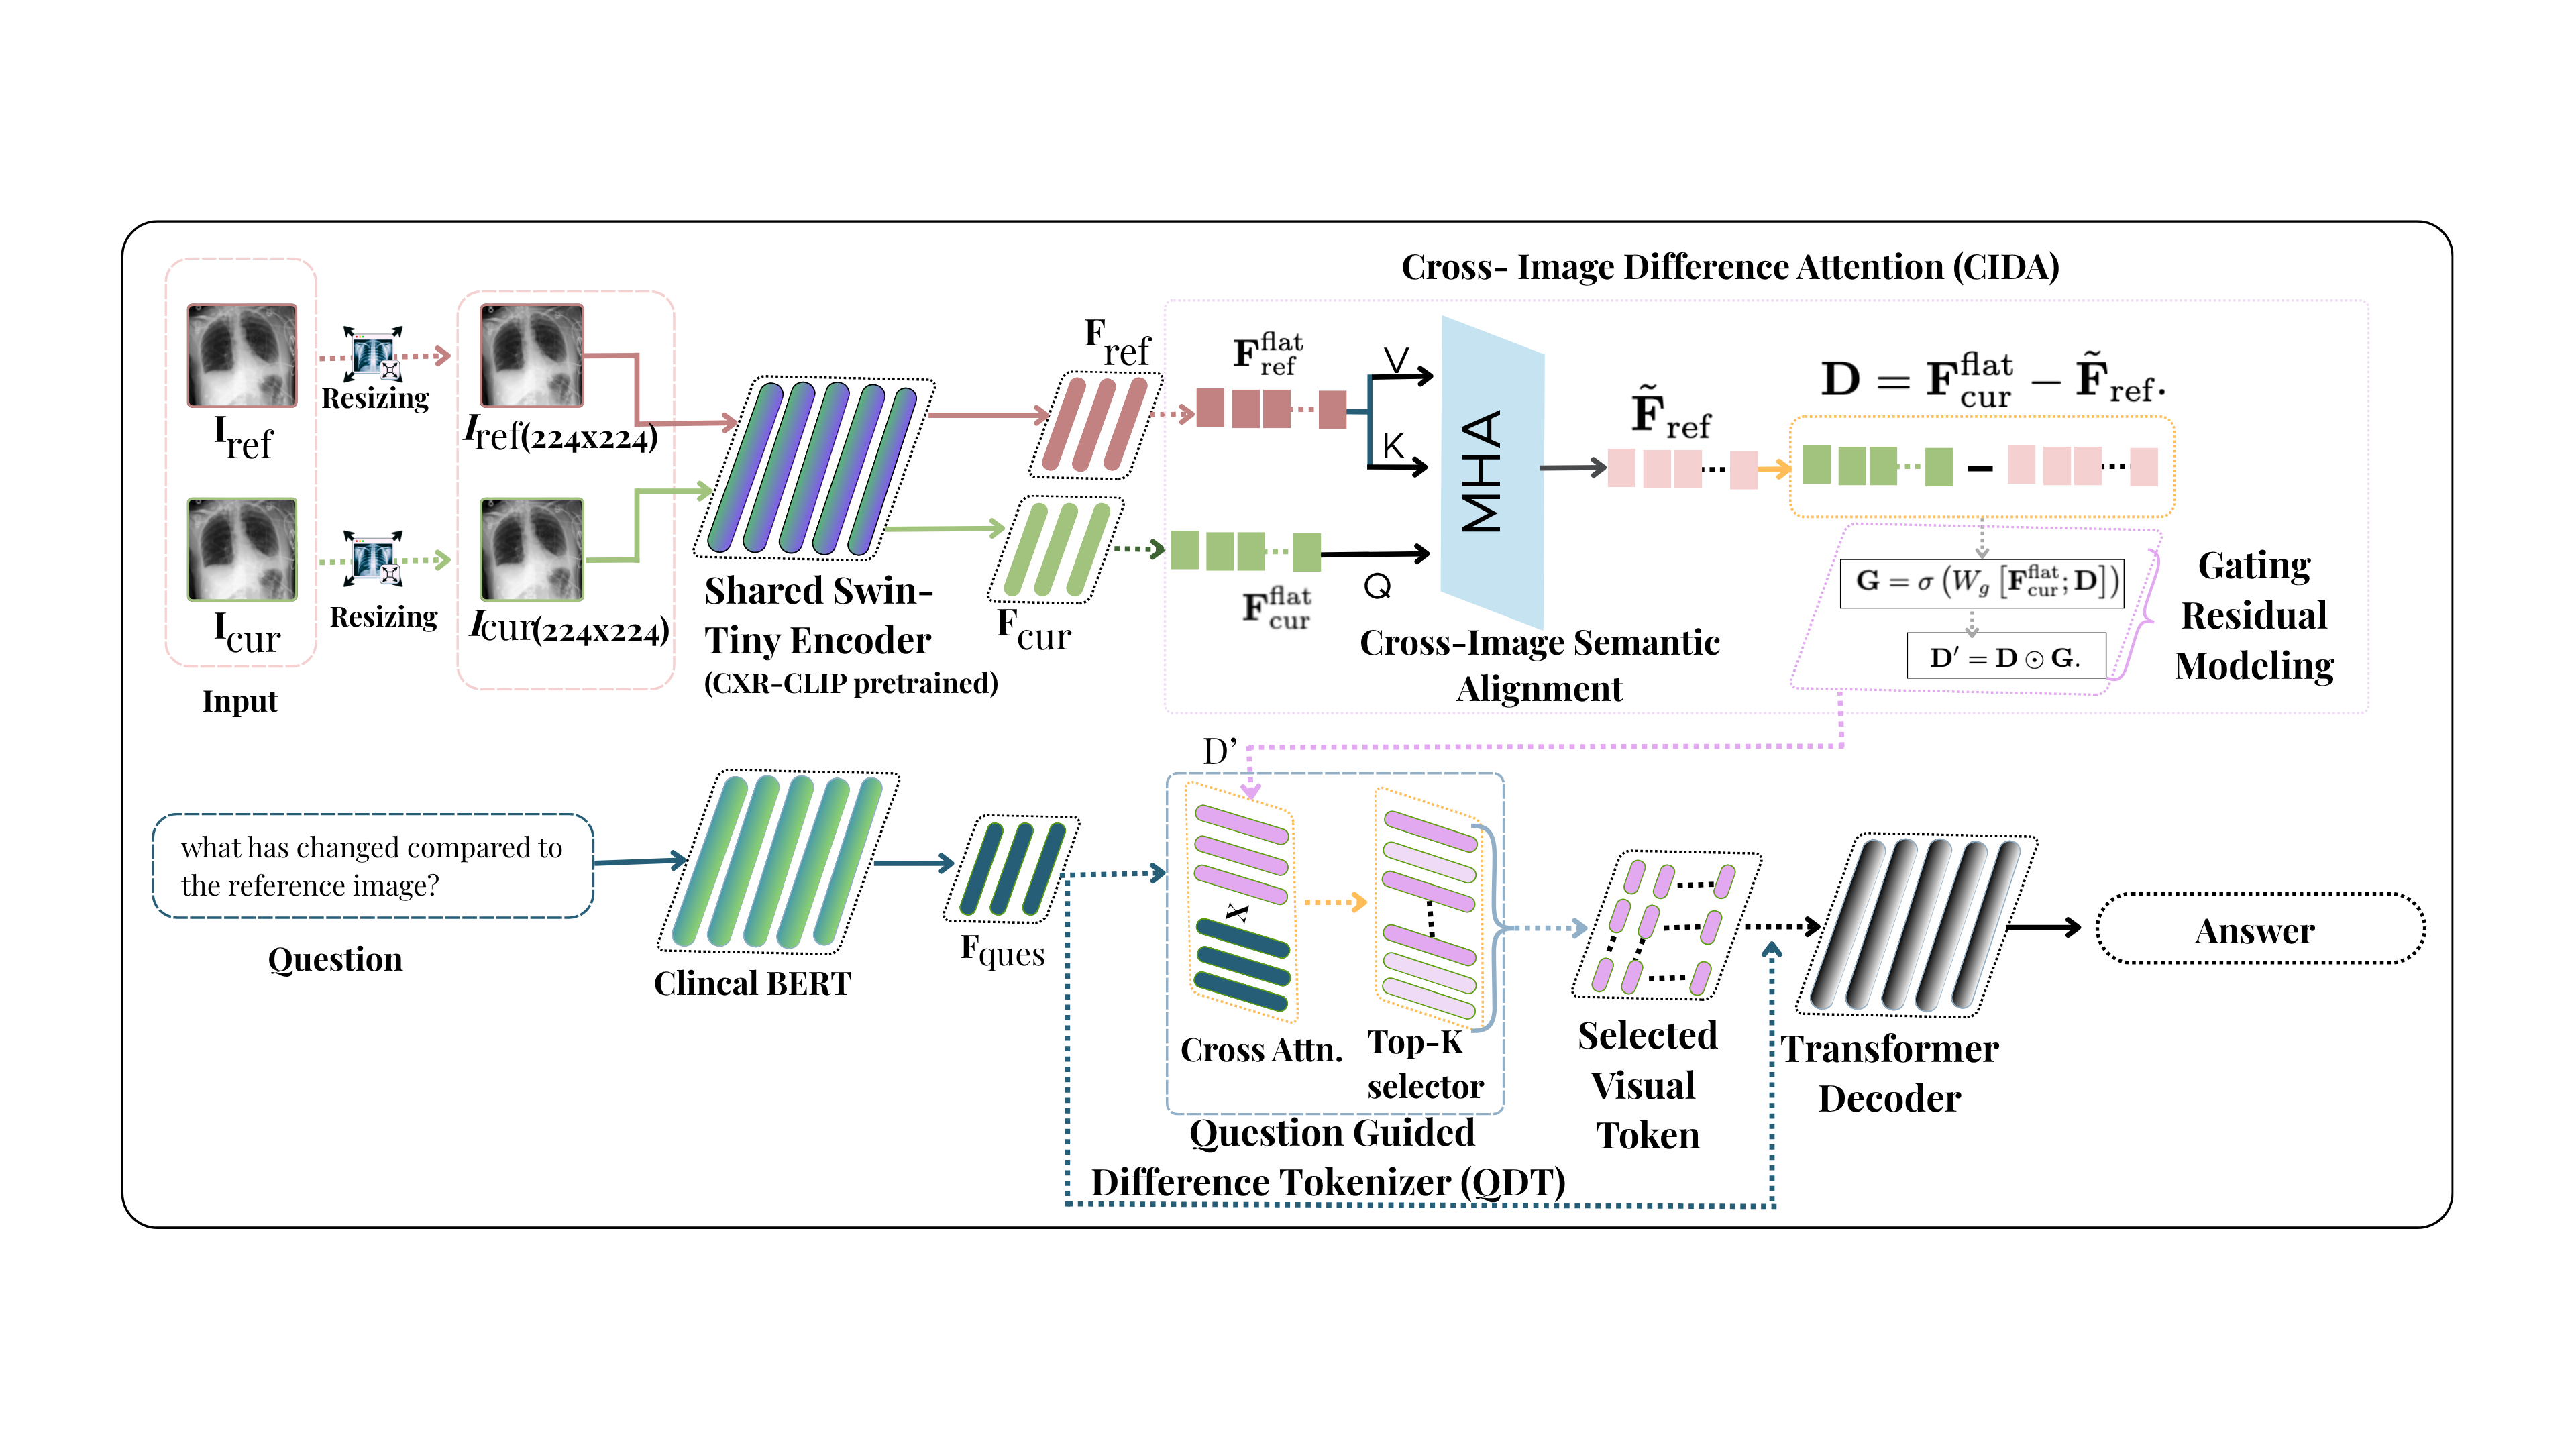
\includegraphics[width=0.9\textwidth]{figures/high_architecture.png}
	\caption{High Level Architecture Overview}
	\label{fig:high_architecture}
\end{figure}

As illustrated in Figure \ref{fig:high_architecture}, the proposed methodology shifts from a brute-force comparison paradigm to an efficient, explicit reasoning framework. The architecture is composed of three primary functional blocks. Cross-Image Difference Attention (CIDA) and gated residual modeling semantically reconstructs and aligns historical features to the current scan before isolating evolution-aware deviations. Question-Guided Difference Tokenizer (QDT) employs cross-attention to selectively pool a sparse, highly relevant set of temporal changes based on the clinical query. Conditional answer generation and multi-stage training utilizes a lightweight transformer decoder optimized through a highly structured multi-stage training strategy to ensure grounded, halucination-free reasoning.

\section{Problem Formulation}
Given a patient's historical reference X-ray $I_{ref}$, a current follow-up X-ray $I_{cur}$, and a clinically grounded question $Q$, the objective of the Diff-VQA system is to generate an accurate natural language answer $\hat{A}$ describing the temporal evolution of the targeted pathology. Instead of mapping inputs directly to a dense difference map, our formulation isolates question-relevant residual deviations to conditionally autoregress the answer.

\section{Architectural Components}

\subsection{Visual Feature Extraction}
The visual processing pipeline begins by encoding the paired longitudinal images. Both $I_{ref}$ and $I_{cur}$ are resized to $224 \times 224$ and passed through a shared tiny variant of \cite{swin}. The shifted-window self-attention mechanism within the encoder enables highly efficient local-to-global context modeling. To inject domain-specific radiographic priors immediately into the feature extraction phase, the backbone is initialized with pretrained weights from \cite{cxr-clip}. This process yields two feature maps, which are flattened into token sequences:
\begin{equation}
	F_{ref}^{flat}, F_{cur}^{flat} \in \mathbb{R}^{B \times N \times C}
\end{equation}
where $B$ is the batch size, $C$ is the channel dimension, and $N = H \times W$ represents the number of spatial patches.

\subsection{Cross Image Difference Attention}
To compensate for spatial misalignments resulting from varying patient positioning and inspiratory effort between visits, we introduce the CIDA module. It utilizes Multi-Head Cross-Attention (MHA) to semantically align the historical features to the coordinate space of the current image. Specifically, the current image features are utilized as queries ($Q$), while the reference image features serve as keys ($K$) and values ($V$):
\begin{equation}
	\tilde{F}_{ref} = \text{MHA}(F_{cur}^{flat}, F_{ref}^{flat}, F_{ref}^{flat})
\end{equation}
This operation reconstructs an aligned historical representation ($\tilde{F}_{ref}$) that is spatially coherent with the current scan, creating a reliable foundation for calculating true temporal differences.

\subsection{Learnable Gated Residual Modeling}
Once the features are aligned, the raw residual deviation is computed via element-wise subtraction:
	\begin{equation}
		D = F_{cur}^{flat} - \tilde{F}_{ref}
	\end{equation}
Because medical imaging inherently contains acquisition noise, utilizing the raw residual $D$ directly can mislead downstream modules. Therefore, a learnable gating mechanism is applied. The gate calculates a channel-wise importance filter by concatenating the current features with the raw residual and passing them through a projection matrix $W_g$ and a sigmoid function $\sigma$:
	\begin{equation}
		G = \sigma(W_g[F_{cur}^{flat} ; D])
	\end{equation}
The refined, evolution-aware residual features are then extracted via element-wise multiplication:
	\begin{equation}
		D' = D \odot G
	\end{equation}
The resulting tokens $\{D'_i\}_{i=1}^N$ encode clean, structured temporal changes.

\subsection{Domain-Aware Text Encoding}
The clinical question $Q$ is encoded using \cite{bio-clinical-bert}, a language model extensively pretrained on clinical notes. This provides a domain-aware question embedding vector $F_{ques} \in \mathbb{R}^C$ that captures the semantic nuance of radiological terminology such as distinguishing between consolidation and atelectasis.

\subsection{Question-Guided Difference Tokenization}
Standard Diff-VQA models process all spatial tokens, which dilutes the signal of localized pathologies. The QDT module solves this by selectively pooling only the temporal changes that are relevant to the specific clinical question.Attention weights ($\alpha_i$) are computed between the question embedding $F_{ques}$ and each visual residual token $D'_i$ using dot-product attention. To enforce extreme token sparsity and computational efficiency, a hard Top-K selection mechanism is applied:
\begin{equation}
	T_{vis} = \text{TopK}(\{\alpha_i D'_i\})
\end{equation}
Based on empirical ablations, $K$ is set to 16, ensuring the model forwards only the most highly discriminative visual evidence to the language decoder.

\subsection{Conditional Answer Generation}
The final response generation relies on a lightweight standard transformer decoder. The selected sparse visual tokens $T_{vis}$ are concatenated with the question embedding $F_{ques}$. The decoder autoregressively predicts the answer $\hat{A}$ step-by-step, conditioned strictly on the question semantics and the isolated, aligned temporal changes.

\subsection{Counterfactual Regularizer}
To mitigate the model's tendency to hallucinate, a counterfactual regularizer (CFA-Reg) is introduced. For each training sample $(I_{cur},I_{ref}, Q, A)$, we generate a logical opposite by either swapping the images $(I_{ref},I_{cur})$ or negating a directional term in the question (e.g., "worsened" → "improved"). The model performs a forward pass on both the real and counterfactual inputs, generating two distinct answer distributions, $P_{real}$ and $P_{cofa}$.


\subsection{Masked Residual Modeling}
The masked residual modeling (MRM) process is designed to force the model to learn the contextual structure of the difference maps. First, an unlabeled image pair $(I_{cur}, I_{ref})$ is passed through the vision encoder to generate the concatenated residual map, $R$. A significant portion of the patches in this map are then randomly masked. The unmasked patches are fed into the QDT's vision backbone, which is tasked with predicting the content of the masked patches. Figure \ref{fig:mrm} shows architecture of masked residual modeling module. 


The training of MRM is guided by a reconstruction loss, which measures the dissimilarity between the model's predicted patches and the original, unmasked patches. We use a Mean Squared Error (MSE) loss for this objective.

$$
L_{\text{MRM}} = \frac{1}{|M|} \sum_{i \in M} (R_{i}^{*} - \hat{R}_{i}^{*})^{2}
$$

Here, M is the set of masked patch indices, $R_i$ is the original patch, and 
$\hat{R}_i$ is the reconstructed patch.
 
\begin{figure}[htbp]
	\centering
	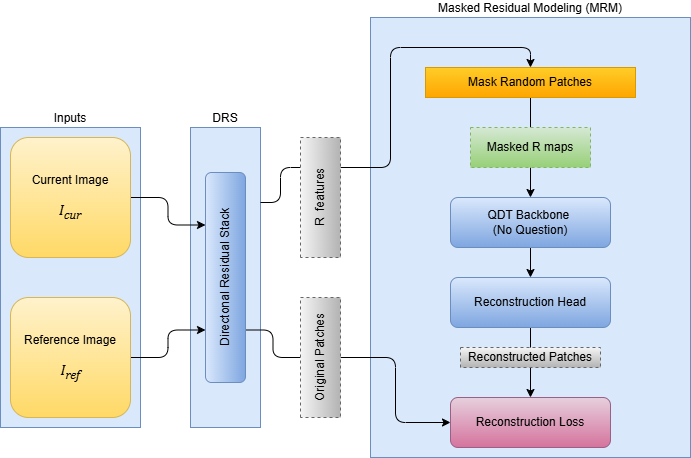
\includegraphics[width=0.9\textwidth]{figures/mrm.png}
	\caption{Masked Residual Modeling}
	\label{fig:mrm}
\end{figure}

\section{Multi-Stage Training Strategy}
The model is optimized using a comprehensive four-stage training regimen to ensure model robustness, prevent shortcut learning, and explicitly ground the vision-language alignment, 

To enforce contextual coherence in the visual representation, 50 percent of the residual tokens are randomly masked in the first stage. A lightweight reconstructor is trained to predict the masked tokens from the visible context using a Mean Squared Error (MSE) objective ($\mathcal{L}_{mrm}$). 

In second stage, a multi-label classification head is attached to predict 14 standard thoracic diseases from both the reference and current features using a Binary Cross-Entropy loss ($\mathcal{L}_{cls}$) to explicitly ground the visual features in known pathology 

To mitigate spurious correlations and dataset biases and hallucinations, the model applies a combination of hierarchical Kullback-Leibler (KL) divergence and Noise Contrastive Estimation (NCE) in third stage. By contrasting true longitudinal pairs against synthetically perturbed counterfactual pairs, the model disentangles true temporal evolution from visual noise ($\mathcal{L}_{cf}$). 

In the last stage, the entire architecture is fine-tuned for the generation task using a standard language cross-entropy loss ($\mathcal{L}_{lang}$) alongside an L1 sparsity regularization penalty on the gating weights ($\mathcal{L}_{gate}$) to force the gate to actively suppress non-essential information. The total loss of the complete training objective is weighted sum of these components.
\begin{equation}
	\mathcal{L}_{total} = \lambda_{lang}\mathcal{L}_{lang} + \lambda_{gate}\mathcal{L}_{gate} + \lambda_{mrm}\mathcal{L}_{mrm} + \lambda_{cls}\mathcal{L}_{cls} + \lambda_{cf}\mathcal{L}_{cf}
\end{equation}

\section{Implementation Details}
To ensure full reproducibility, ALIGN-VQA was developed using \cite{pytorch}. The model features a highly efficient parameter footprint of approximately 182.5M parameters. The QDT module retains a maximum of 64 tokens during early training, which is dynamically pruned to $K=16$ during fine-tuning. The maximum generated answer length is constrained to 128 tokens. Optimization is performed using the AdamW optimizer with a batch size of 128 and an initial learning rate of $5 \times 10^{-5}$, governed by a cosine annealing learning rate scheduler. The training schedule consists of 1 epoch of MRM, 3 warm-up epochs, and 20 epochs of end-to-end VQA fine-tuning. The empirically derived loss weights are set to $\lambda_{lang}=1.0$, $\lambda_{mrm}=0.1$, $\lambda_{cf}=0.1$, and $\lambda_{cls}=0.5$. Vocabulary mismatch issues during inference are handled dynamically by matching the initialized target vocabulary dimension to the exact embedding size preserved in the saved model checkpoints.

\setlength{\footskip}{8mm}

\chapter{EXPERIMENTS}


\section{Rationale}
The primary objective of these experiments is to rigorously evaluate the clinical viability, computational efficiency, and reasoning accuracy of the proposed ALIGN-VQA architecture. Traditional Medical Visual Question Answering (Med-VQA) models often falter when applied to longitudinal tasks because they are vulnerable to spatial misalignments and struggle to isolate true disease progression from harmless acquisition noise. Therefore, the experimental design is motivated by three key goals. First, the author argues that spatial misalignments and stochastic acquisition variability between historical and current scans compromise direct feature comparison. Thus, the Cross-Image Difference Attention (CIDA) module is evaluated on its ability to semantically reconstruct and align the prior-visit features to establish a reliable, misalignment-tolerant baseline. Second, rather than assuming all raw pixel-wise differences are clinically relevant, the author hypothesizes that a Learnable Residual Gating mechanism is required to actively filter out non-pathological visual noise and static anatomy, ensuring that only precise, evolution-aware features are extracted. Finally, because the vast majority of regions in a longitudinal chest X-ray remain unchanged, the author evaluates the Question-Guided Difference Tokenizer (QDT) to determine if selectively pooling a sparse subset of highly relevant tokens enables the model to perform targeted diagnostic reasoning while maintaining a highly efficient, lightweight architecture.


\section{Dataset}
To test these hypotheses, the author utilizes \cite{medical-diff-vqa}, which is a specialized derivative of the large-scale \cite{mimic-cxr}. Each sample in this dataset is structured as a longitudinal pair consisting of a historical reference radiograph and a more recent follow-up scan, stored in Digital Imaging and Communications in Medicine (DICOM) format. The x-rays images in Joint Photographic Experts Group (JPEG) format are fetched from \cite{mimic-cxr-jpg} for faster preprocessing and training. These pairs are accompanied by clinically grounded questions that specifically target temporal changes, such as the progression of pleural effusion or the placement of medical devices. The dataset comprises 164,324 pairs of main and reference chest X-ray images, yielding a total of 700,703 question-answer pairs. This high volume of data allows the model to learn the subtle semantic nuances required to distinguish between common clinical conditions like consolidation, edema, and atelectasis within a comparative context. Following standard benchmarking protocols, the dataset is strictly partitioned into training, validation, and testing sets using an 8:1:1 ratio. The Figure shows the distribution of seven distinct clinical categories

\subsection{Pathological Distribution}
Figure \ref{fig:medical_findings} illustrates the prevalence of medical findings across the dataset. The distribution exhibits a heavy long-tail characteristic typical of medical datasets. "No Finding" and "Support Devices" are the most prevalent positive labels, reflecting the high frequency of routine exams and Intensive Care Unit (ICU) patient monitoring in \cite{mimic-cxr}. Among true pathological findings, "Pleural Effusion," "Lung Opacity," and "Atelectasis" occur most frequently. Conversely, critical but less frequent findings like "Fracture" and "Pleural Other" appear significantly less often. This class imbalance highlights the necessity for robust representation learning, particularly the Counterfactual Regularizer in the ALIGN-VQA architecture, to prevent the model from defaulting to high-frequency predictions.

\begin{figure}[htbp]
	\centering
	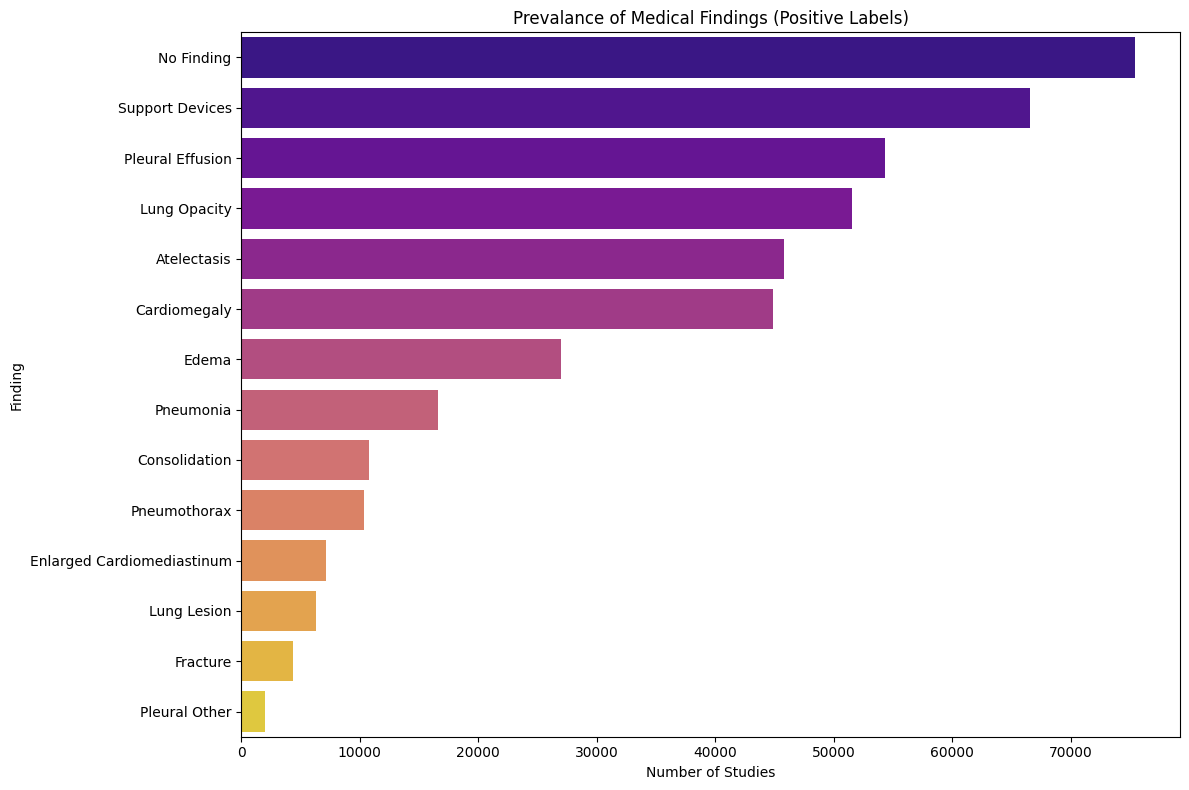
\includegraphics[width=0.9\textwidth]{figures/medical_findings.png}
	\caption{Prevalance of Medical Findings}
	\label{fig:medical_findings}
\end{figure}

\subsection{Question Type Distribution}
The questions are categorized into seven distinct clinical types, as shown in Figure \ref{fig:question_types}. The distribution is relatively balanced among the top categories, ensuring a diverse evaluation of the model's capabilities. The "Difference" category is the most frequent accounting for approximately 23 percent of the dataset, followed closely by "Presence", 22 percent and "Abnormality" 21 percent. The remaining categories—Location, Level, View, and Type—make up the rest of the dataset. While the ALIGN-VQA model is trained and evaluated across all seven categories, the primary focus of these experiments remains the "Difference" subset, as it explicitly tests the model's ability to reason about longitudinal spatial and pathological changes between the reference and current scans.

\begin{figure}[htbp]
	\centering
	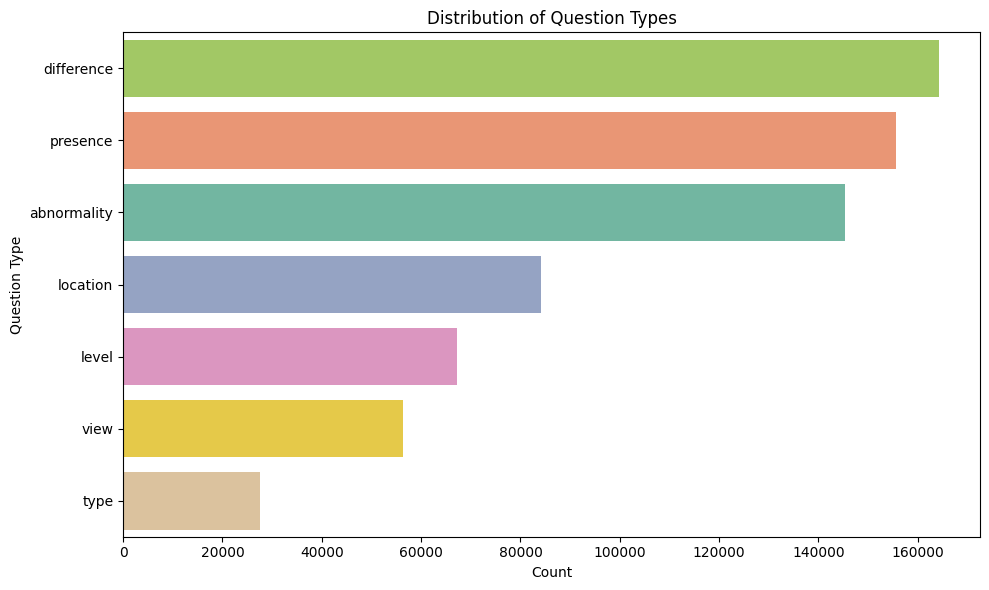
\includegraphics[width=0.9\textwidth]{figures/question_types.png}
	\caption{Distribution of Question Types}
	\label{fig:question_types}
\end{figure}

\subsection{Linguistic Distribution}
Figure \ref{fig:question_lengths} visualizes the distribution of question and answer lengths in characters. The question lengths exhibit a highly structured, multi-modal distribution with distinct peaks around 30, 42, and 50 characters. This rigid structure suggests that the questions were generated using a programmatic or templated approach based on the original radiology reports, rather than free-form human querying. The answer lengths are heavily skewed, with the vast majority of answers being extremely concise, under 25 characters, corresponding to binary "yes/no" answers or short categorical responses. A smaller, secondary distribution of longer answers, 50 to 150 characters, corresponds to the complex, descriptive answers required for the "Difference" and "Abnormality" question types.

\begin{figure}[htbp]
	\centering
	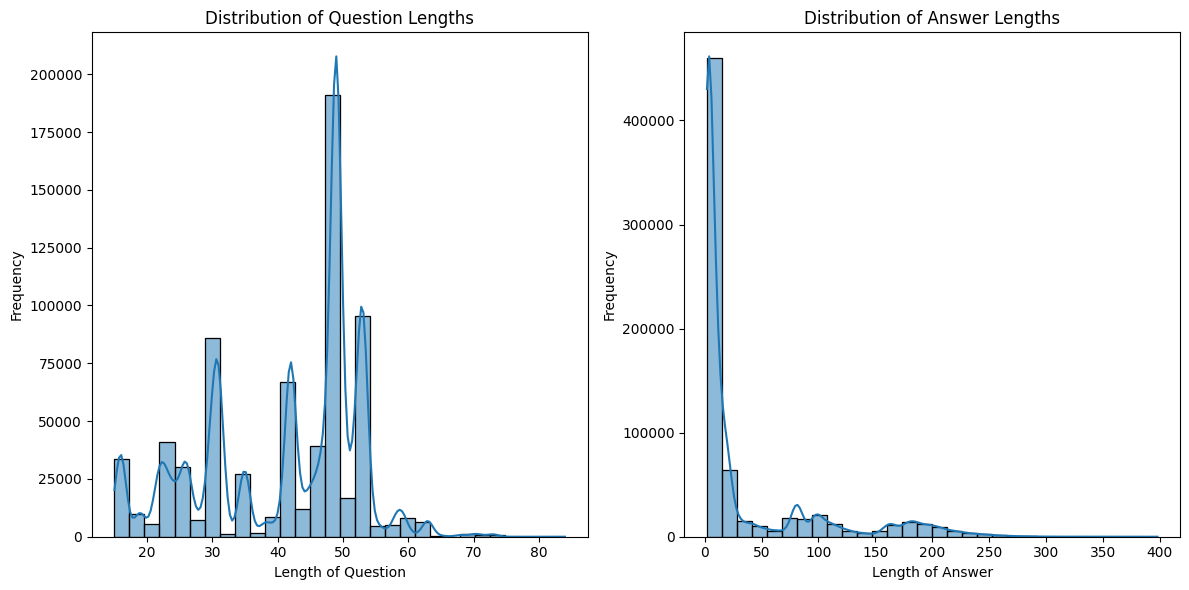
\includegraphics[width=0.9\textwidth]{figures/question_lengths.png}
	\caption{Distribution of Question Lengths}
	\label{fig:question_lengths}
\end{figure}


\section{Experiment Setting}

\subsection{Preprocessing}
To ensure standardized inputs for the vision-language pipeline, rigorous preprocessing protocols were applied to both the imaging and textual data. The resizing pipeline is engineered to maximize computational efficiency while preserving critical clinical details. Both historical and current chest X-rays were resized to $224 \times 224$ pixels to match the input dimensions expected by the tiny varient of \cite{swin}. Standard normalization was applied using \cite{cxr-clip} pretraining statistics to ensure stable feature extraction. Clinical questions were tokenized using \cite{bio-clinical-bert}, with sequences padded and truncated to a maximum length of 48 tokens. To prevent index-out-of-bounds errors and size mismatches during evaluation, a common issue when dataset splits yield varying unique word counts, the inference scripts were programmed to dynamically extract the exact expected vocabulary size directly from the saved model checkpoints prior to initializing the classification head.

\subsection{Models and Techniques}
To benchmark the proposed ALIGN-VQA architecture, its performance is compared against several state-of-the-art models that encompass both general domain change-captioning and specialized medical Diff-VQA. Among the specialized medical models, the author evaluates \cite{ekaid}, a foundational Diff-VQA framework that relies on pre-extracted bounding boxes and an anatomical knowledge graph to model changes. The author also compares the method with \cite{plural}, a computationally intensive transformer framework that utilizes massive external pretraining on natural images and radiology reports to process dense, unpruned feature concatenations. Additionally, the author benchmarks against \cite{regiomix}, a Retrieval-Augmented Generation (RAG) approach that generates pseudo-difference descriptions by mixing and matching retrieved regions from an external database. Furthermore, the author includes two recent generative medical VQA architectures including \cite{real}, which employs a dedicated residual encoder and residual feature alignment to capture image disparities, and \cite{encoder-decoder}, which utilizes \cite{swin} coupled with image differentiation embeddings to distinguish temporal scans prior to decoding.

Against these baselines, the author evaluate the proposed ALIGN-VQA, an alignment-guided residual modeling architecture featuring CIDA, a learnable gating mechanism, and the QDT. Beyond direct comparisons, extensive ablation studies are conducted on ALIGN-VQA by systematically toggling key components. For instance, the CIDA module is disabled to force direct feature subtraction, and the QDT Top-K selection threshold is altered. This allows the author to rigorously isolate and quantify the individual contributions of these novel mechanisms to the overall diagnostic accuracy.

\subsection{Training Procedure}
The model was implemented in \cite{pytorch} and trained end-to-end to ensure full reproducibility. All training procedures were executed on NVIDIA RTX6000 to efficiently accommodate the required batch sizes and the computational overhead of the attention matrix operations. The network was optimized using the AdamW optimizer with a batch size of 128. To ensure smooth convergence, the initial learning rate was set to $5 \times 10^{-5}$ and governed by a cosine annealing scheduler.

The training process strictly adhered to a multi-stage strategy designed to incrementally build the model's reasoning capabilities. This schedule commenced with one initial epoch of self-supervised Masked Residual Modeling (MRM), followed by three warm-up epochs, and concluded with 20 epochs of end-to-end Diff-VQA fine-tuning. The compound loss function was balanced using empirically derived weights, applying a weight of 1.0 to the language generation loss, 0.1 to the MRM loss, 0.1 to the counterfactual loss, and 0.5 to the auxiliary classification loss. Finally, early stopping was implemented based on validation CIDEr scores to continually monitor generalization and prevent overfitting during the fine-tuning phase.

\subsection{Evaluation Metrics}
Because automated metrics often struggle to capture the clinical nuance of medical texts, the evaluation strategy utilizes a robust mix of strict string-matching, semantic similarity, and human validation. For automated assessment, the author reports standard Natural Language Generation (NLG) metrics, including \cite{bleu}, \cite{meteor}, and \cite{rouge}, to evaluate sequence overlap and structural fluency. The author places a heavy priority on the \cite{cider} metric, as its weighting mechanism explicitly penalizes generic answers and rewards the accurate generation of rare, clinically vital keywords, such as specific pathology names.

\begin{comment}

\section{Quantitative Results on the MIMIC-Diff-VQA Benchmark}
Table 5.1 presents the quantitative performance of the proposed ALIGN-VQA against current state-of-the-art models on the \cite{medical-diff-vqa}. The evaluated baselines include early graph-based methods, retrieval-augmented models, dense-feature frameworks, and residual-based generative models.

As the results indicate, while models like \cite{encoder-decoder} and \cite{real} achieve marginally higher scores on strict n-gram overlap metrics, the proposed model establishes a new state-of-the-art on the most clinically vital metrics: \cite{meteor} (0.480), \cite{rouge} (0.739), and \cite{cider} (2.427). This distinction is critical. \cite{bleu} uniformly weights all words, heavily rewarding the generation of common syntax templates. In contrast, \cite{cider} penalizes generic, high-frequency phrases while heavily rewarding the accurate prediction of rare, informative keywords such as specific pathology names or directional clinical terms. ALIGN-VQA’s dominant \cite{cider} score of 2.427—outperforming the highly competitive \cite{real} (2.409) and vastly exceeding dense-feature models like \cite{encoder-decoder} (2.119) and \cite{plural} (1.832)—demonstrates that the extreme, QDT successfully filters out background noise without losing crucial diagnostic indicators.

\section{Ablation Studies and Component Analysis}
To isolate the contributions of the core architectural innovations, the author conducted extensive ablation studies, the results of which are detailed in Table 5.2. We evaluated the model by systematically toggling the CIDA module, CF-Reg, and varying the Top-$k$ threshold in the QDT.

\subsection{Impact of Architectural Modules}
The baseline configuration without CIDA and CF-Reg performs poorly, yielding \cite{cider} of just 1.213. Introducing the CF-Reg alone improves the metric to 1.956, confirming its role in mitigating hallucinations. Conversely, introducing CIDA alone (Row 4) significantly boosts the metric to 2.172, providing empirical proof that explicitly resolving spatial misalignment before calculating residuals is far superior to direct feature subtraction. Combining both modules yields the optimal the score of 2.427, demonstrating that robust spatial alignment and causal, hallucination-free reasoning are highly complementary.

\subsection{Impact of Token Sparsity}
The author also investigated the effect of the token selection threshold, $k$, within the QDT module. Setting $k$ too low ($k=12$) limits the visual evidence available to the language decoder, dropping \cite{cider} to 2.258. Conversely, increasing the threshold ($k=49$) incorporates excessive visual noise and irrelevant anatomical changes, diluting the clinical signal and lowering the metric to 2.226. The empirical sweet spot of $k=16$ ensures that the model remains highly focused on the exact pathological deviations referenced by the clinical question.

\begin{table}[htbp]
	\centering
	\caption{Quantitative performance comparison of the proposed model against state-of-the-art methods on the MIMIC-Diff-VQA dataset.}
	\label{tab:main_results_old}
	\renewcommand{\arraystretch}{1.2}
	% Resizebox scales the table to perfectly fit the text width
	\resizebox{\textwidth}{!}{%
		\begin{tabular}{l ccccccc}
			\toprule
			\textbf{Model} & \textbf{BLEU-1} & \textbf{BLEU-2} & \textbf{BLEU-3} & \textbf{BLEU-4} & \textbf{METEOR} & \textbf{ROUGE-L} & \textbf{CIDEr} \\
			\midrule
			\cite{ekaid}    & 0.624 & 0.541 & 0.477 & 0.422 & 0.337 & 0.645 & 1.893 \\
			\cite{regiomix} & 0.705 & 0.633 & 0.572 & 0.517 & 0.381 & 0.651 & 1.804 \\
			\cite{plural}   & 0.704 & 0.633 & 0.575 & 0.520 & 0.381 & 0.653 & 1.832 \\
			\cite{encoder-decoder}      & 0.716 & 0.647 & 0.590 & 0.537 & 0.389 & 0.670 & 2.119 \\
			\cite{real}     & 0.710 & 0.636 & 0.580 & 0.530 & 0.395 & 0.736 & 2.409 \\
			%MENDER   & 0.635 & 0.568 & 0.518 & 0.457 & 0.354 & 0.615 & 1.684 \\
			\midrule
			\textbf{Ours} & \textbf{0.653} & \textbf{0.578} & \textbf{0.518} & \textbf{0.466} & \textbf{0.480} & \textbf{0.739} & \textbf{2.427} \\
			\bottomrule
		\end{tabular}%
	}
\end{table}

\begin{table}[htbp]
	\centering
	\caption{Ablation studies isolating the impact of the Top-$k$ selection threshold, Cross-Image Difference Attention (CIDA), and Counterfactual (CF) regularizer.}
	\label{tab:ablation_old}
	\renewcommand{\arraystretch}{1.2}
	% Resizebox scales the table to perfectly fit the text width
	\resizebox{\textwidth}{!}{%
		\begin{tabular}{c c c ccccc c c}
			\toprule
			\textbf{Top-$k$} & \textbf{CIDA} & \textbf{CF} & \textbf{BLEU-1} & \textbf{BLEU-2} & \textbf{BLEU-3} & \textbf{BLEU-4} & \textbf{METEOR} & \textbf{ROUGE-L} & \textbf{CIDEr} \\
			\midrule
			12 & $\checkmark$ & $\checkmark$ & 0.636 & 0.541 & 0.502 & 0.450 & 0.481 & 0.700 & 2.258 \\
			49 & $\checkmark$ & $\checkmark$ & 0.631 & 0.555 & 0.496 & 0.445 & 0.480 & 0.713 & 2.226 \\
			16 & $\times$     & $\times$     & 0.399 & 0.340 & 0.296 & 0.256 & 0.274 & 0.485 & 1.213 \\
			16 & $\checkmark$ & $\times$     & 0.643 & 0.565 & 0.504 & 0.453 & 0.457 & 0.660 & 2.172 \\
			16 & $\times$     & $\checkmark$ & 0.661 & 0.577 & 0.511 & 0.453 & 0.454 & 0.661 & 1.956 \\
			\midrule
			\textbf{16} & $\checkmark$ & $\checkmark$ & \textbf{0.653} & \textbf{0.578} & \textbf{0.518} & \textbf{0.466} & \textbf{0.480} & \textbf{0.739} & \textbf{2.427} \\
			\bottomrule
		\end{tabular}%
	}
\end{table}

\end{comment}
\setlength{\footskip}{8mm}

\chapter{RESULTS}
	
It is essential to establish the analytical framework used to evaluate the proposed ALIGN-VQA architecture before detailing empirical findings. The primary objective of these experiments is to rigorously evaluate the clinical viability, computational efficiency, and reasoning accuracy of the model.

To conduct a comprehensive analysis, the author utilized \cite{bleu} to measure precise structural n-gram overlap, \cite{rouge} to evaluate the preservation of the chronological clinical narrative, \cite{meteor} to account for valid semantic synonyms, and \cite{cider} to measure the model’s ability to capture high-value, rare diagnostic keywords. Additionally, \cite{bert-score} was employed to assess deep semantic similarity. The results are structurally aligned with the three core research questions, analyzing the model sequentially through its forward-pass pipeline: establishing spatial alignment, filtering non-pathological noise, and performing targeted token reasoning.

Table \ref{tab:main_results} presents the quantitative performance of the proposed ALIGN-VQA against current state-of-the-art models on the \cite{medical-diff-vqa}. The evaluated baselines include early graph-based methods, retrieval-augmented models, dense-feature frameworks, and residual-based generative models. To isolate the contributions of the core architectural innovations, the author conducted extensive ablation studies, the results of which are detailed in Table \ref{tab:ablation}. The author evaluated the model by systematically toggling the Cross Image Difference Attention (CIDA) module, Learnable Residual Gating Mechanism (GATE), and varying the Top-$k$ threshold in the Question-Guided Difference Tokenizer (QDT).

\begin{table}[htbp]
	\centering
	\caption{Quantitative performance comparison of the proposed model against state-of-the-art methods on \cite{medical-diff-vqa}.}
	\label{tab:main_results}
	\renewcommand{\arraystretch}{1.2}
	% Resizebox scales the table to perfectly fit the text width
	\resizebox{\textwidth}{!}{%
		\begin{tabular}{l ccccccc}
			\toprule
			\textbf{Model} & \textbf{BLEU-1} & \textbf{BLEU-2} & \textbf{BLEU-3} & \textbf{BLEU-4} & \textbf{METEOR} & \textbf{ROUGE-L} & \textbf{CIDEr} \\
			\midrule
			\cite{ekaid}    & 0.624 & 0.541 & 0.477 & 0.422 & 0.337 & 0.645 & 1.893 \\
			\cite{regiomix} & 0.705 & 0.633 & 0.572 & 0.517 & 0.381 & 0.651 & 1.804 \\
			\cite{plural}   & 0.704 & 0.633 & 0.575 & 0.520 & 0.381 & 0.653 & 1.832 \\
			\cite{encoder-decoder}      & 0.716 & 0.647 & 0.590 & 0.537 & 0.389 & 0.670 & 2.119 \\
			\cite{real}     & 0.710 & 0.636 & 0.580 & 0.530 & 0.395 & 0.736 & 2.409 \\
			%MENDER   & 0.635 & 0.568 & 0.518 & 0.457 & 0.354 & 0.615 & 1.684 \\
			\midrule
			\textbf{ALIGN-VQA} & \textbf{0.653} & \textbf{0.578} & \textbf{0.518} & \textbf{0.466} & \textbf{0.480} & \textbf{0.739} & \textbf{2.427} \\
			\bottomrule
		\end{tabular}%
	}
\end{table}

\begin{table}[htbp]
	\centering
	\caption{Ablation studies isolating the impact of the Top-$k$ selection threshold, CIDA, and GATE.}
	\label{tab:ablation}
	\renewcommand{\arraystretch}{1.2}
	% Resizebox scales the table to perfectly fit the text width
	\resizebox{\textwidth}{!}{%
		\begin{tabular}{c c c c c c c c c c c}
			\toprule
			\textbf{Top-$k$} & \textbf{CIDA} & \textbf{GATE} & \textbf{BLEU-1} & \textbf{BLEU-2} & \textbf{BLEU-3} & \textbf{BLEU-4} & \textbf{METEOR} & \textbf{ROUGE-L} & \textbf{CIDEr} & \textbf{BERT-F1} \\
			\midrule
			12 & $\times$     & $\times$     & 0.566 & 0.493 & 0.437 & 0.386 & 0.414 & 0.635 & 1.757 & 0.833 \\
			12 & $\times$     & $\checkmark$ & 0.625 & 0.551 & 0.493 & 0.442 & 0.416 & 0.624 & 1.853 & 0.844 \\
			12 & $\checkmark$ & $\times$     & 0.623 & 0.553 & 0.499 & 0.449 & 0.459 & 0.676 & 2.118 & 0.849 \\
			12 & $\checkmark$ & $\checkmark$ & 0.636 & 0.541 & 0.502 & 0.450 & 0.481 & 0.700 & 2.258 & 0.952 \\
			\midrule
			49 & $\times$     & $\times$     & 0.600 & 0.527 & 0.470 & 0.420 & 0.416 & 0.619 & 1.923 & 0.942 \\
			49 & $\checkmark$ & $\times$     & 0.669 & 0.591 & 0.532 & 0.480 & 0.462 & 0.665 & 2.089 & 0.947 \\
			49 & $\times$     & $\checkmark$ & 0.566 & 0.500 & 0.449 & 0.406 & 0.411 & 0.611 & 1.915 & 0.941 \\
			49 & $\checkmark$ & $\checkmark$ & 0.631 & 0.555 & 0.496 & 0.445 & 0.480 & 0.713 & 2.226 & 0.948 \\
			\midrule
			16 & $\times$     & $\times$     & 0.215 & 0.165 & 0.134 & 0.108 & 0.306 & 0.490 & 1.383 & 0.816 \\
			16 & $\checkmark$ & $\times$     & 0.643 & 0.565 & 0.504 & 0.453 & 0.457 & 0.660 & 2.172 & 0.875 \\
			16 & $\times$     & $\checkmark$ & 0.661 & 0.577 & 0.511 & 0.453 & 0.454 & 0.661 & 1.956 & 0.887 \\
			\midrule
			\textbf{16} & $\checkmark$ & $\checkmark$ & \textbf{0.653} & \textbf{0.578} & \textbf{0.518} & \textbf{0.466} & \textbf{0.480} & \textbf{0.739} & \textbf{2.427} & \textbf{0.953} \\
			\bottomrule
		\end{tabular}%
	}
\end{table}

\begin{table}[htbp]
	\centering
	\caption{Evaluation scores across different clinical question types using the best performing ALIGN-VQA model (Top-16, CIDA-active, Gate-active).}
	\label{tab:question_types}
	\renewcommand{\arraystretch}{1.2}
	\resizebox{\textwidth}{!}{%
		\begin{tabular}{l c c c c c c c}
			\toprule
			\textbf{Question} & \textbf{BLEU-1} & \textbf{BLEU-2} & \textbf{BLEU-3} & \textbf{BLEU-4} & \textbf{METEOR} & \textbf{ROUGE-L} & \textbf{CIDEr} \\
			\midrule
			difference & 0.663 & 0.589 & 0.528 & 0.473 & 0.659 & 0.624 & 2.177 \\
			presence   & 0.849 & 0.009 & 0.001 & 0.000 & 0.424 & 0.849 & 2.123 \\
			abnormality& 0.605 & 0.520 & 0.518 & 0.414 & 0.367 & 0.599 & 1.904 \\
			location   & 0.616 & 0.489 & 0.359 & 0.275 & 0.540 & 0.668 & 2.496 \\
			level      & 0.653 & 0.007 & 0.001 & 0.000 & 0.395 & 0.598 & 1.984 \\
			view       & 0.979 & 0.965 & 0.098 & 0.001 & 0.649 & 0.982 & 3.343 \\
			type       & 0.706 & 0.008 & 0.001 & 0.000 & 0.360 & 0.720 & 1.900 \\
			\midrule
			\textbf{overall} & \textbf{0.653} & \textbf{0.578} & \textbf{0.518} & \textbf{0.466} & \textbf{0.480} & \textbf{0.739} & \textbf{2.427} \\
			\bottomrule
		\end{tabular}%
	}
\end{table}



\section{Results Corresponding to CIDA}
The first research question investigates how semantic reconstruction via the CIDA module affects the model's robustness to spatial misalignments between historical and current scans. The author hypothesized that establishing a misalignment-tolerant baseline is required before calculating image differences. To evaluate this, the author conducted an ablation study comparing a baseline model utilizing direct feature subtraction against the ALIGN-VQA model equipped with CIDA. The results drawn from the comprehensive ablation studies demonstrate a severe vulnerability in direct subtraction methods.

When observing the model operating with a token pool of 16, the baseline model lacking both CIDA and GATE completely collapsed, achieving CIDEr, \cite{cider},  of just 1.383 and BLEU-4, \cite{bleu}, of 0.108. However, when the CIDA module was activated to semantically align the features prior to comparison, performance surged dramatically. The score of CIDEr improved by +0.789 to reach 2.172, while BLEU-4 improved to 0.453. This massive performance delta mathematically validates Hypothesis 1, proving that raw spatial misalignment is a primary cause of catastrophic failure in longitudinal VQA, and that CIDA successfully reconstructs the features to enable accurate temporal comparison.

\section{Results Corresponding to GATE}
The second research question asks how the application of a learnable residual gating mechanism impacts the model's ability to capture precise pathological deviations. The author hypothesized that filtering out non-pathological noise, such as changes in patient posture or scanner contrast, from the raw residual features would yield higher diagnostic accuracy.

The ablation results on the specific difference question subset strongly support this hypothesis. Even with active CIDA module, processing raw, un-gated residuals resulted in a CIDEr score of 2.081. When GATE was introduced to selectively suppress static anatomy and acquisition artifacts, the CIDEr score increased to 2.177, and the BERT-F1, \cite{bert-score}, score rose from 0.917 to 0.929. This impact is even more pronounced on the overall dataset evaluation. Activating the gating mechanism alongside CIDA pushed the model to its absolute peak performance: a CIDEr score of 2.427 and a ROUGE-L, \cite{rouge}, of 0.739. By comparing the gated vs. un-gated architectures, the author confirms that forcing the language decoder to process noisy subtraction maps degrades clinical accuracy, whereas the gating mechanism successfully isolates the true pathologies.

\section{Results Corresponding to QDT}
The last research question evaluates whether selectively pooling temporal changes via the QDT impacts the model's targeted reasoning and overall efficiency. The author hypothesized that because the vast majority of pixels in a longitudinal chest X-ray remain unchanged, a sparse set of highly relevant tokens is sufficient—and often superior—for answering clinical questions. The author tested the model across three different token densities.

Processing the denser 49 tokens yielded a CIDEr score of 2.226. Pruning the features down to 16 tokens improved the CIDEr score to 2.427. Over-pruning to 12 tokens caused performance to drop to 2.258. These results are highly significant. They prove that retaining too much visual information by processing dense features actually harms the model by introducing distracting, irrelevant visual features. The QDT module at Top-16 perfectly balances computational efficiency with diagnostic accuracy, effectively pruning away the background and forcing the model to focus only on the region of interest dictated by the question.


\section{Further Analysis}
\subsection{Comparison with State of the Art Models}
To validate the overall architecture, ALIGN-VQA was benchmarked against leading state-of-the-art Medical VQA models, including EKAID, RegioMix, PLURAL, VED, and ReAI.
ALIGN-VQA achieved the highest overall performance across the most stringent clinical metrics. Most notably, ALIGN-VQA achieved a CIDEr score of 2.427, outperforming the closest baseline (ReAI at 2.409) and vastly exceeding traditional architectures like EKAID (1.893). Furthermore, ALIGN-VQA secured the highest ROUGE-L score (0.739), indicating that the architecture is superior at preserving the correct chronological and relational structure of the diagnostic narrative compared to existing models.

\subsection{Analyzing Distribution Across Question Types}
Because clinical queries vary drastically in complexity, we further analyzed the performance of the best model (Top-16, CIDA-active, Gate-active) across distinct question categories. The model showed exceptional performance on simpler, highly structured tasks such as view questions (CIDEr: 3.343, BLEU-1: 0.979) and location questions (CIDEr: 2.496).

\subsection{Human Evaluation and Error Analysis}
All test samples are manually evaluated beyond Exact Match (EM). While EM was 51.1\%, manual assessment showed 50\% fully correct, 30\% partially correct, and 20\% incorrect predictions. Partial errors mainly involved incomplete specification or minor lexical variations. Performance was strongest for structured categories (type, view: 93.7\% correct), whereas more complex categories (abnormality, difference) showed greater variability (55.8\% fully correct, 25.0\% partially incorrect, 18.8\% incorrect), reflecting the challenge of fine-grained pathology characterization and comparative reasoning. Importantly, no systematic localization failures were observed, and most errors resulted from partial specification rather than clinically
misleading predictions.

\begin{comment}
First remind your readers how you analyze the data in detail here before jumping to results

\textbf{One good way is to sectionize your result based on your research questions.
}
\textbf{Use tables and figures to help explain your results.   
}

\section{Result Corresponding to RQ1}

Example table (see Table \ref{tab:results1}).

\begin{table}[hbt!]
\caption{Some amazing table that we hope good results}
\resizebox{\columnwidth}{!}{%
\begin{tabular}{lcccccc}
\hline
\multicolumn{1}{c}{\textbf{}}                                & \multicolumn{3}{c}{\textbf{XSUM}}          & \multicolumn{3}{c}{\textbf{SQUAD}}         \\ \cline{2-7} 
\multicolumn{1}{c}{\textbf{Model}}                           & \textbf{R-1} & \textbf{R-2} & \textbf{R-L} & \textbf{R-1} & \textbf{R-2} & \textbf{R-L} \\ \hline
(A) Multi-task + Shared-prefix + Frozen Pretrained           & XXX          & XXX          & XXX          & XXX          & XXX          & XXX          \\
(B) Multi-task + Shared-prefix +Unfrozen Pretrained          & XXX          & XXX          & XXX          & XXX          & XXX          & XXX          \\
(C) Multi-task + Without shared-prefix + Frozen Pretrained   & XXX          & XXX          & XXX          & XXX          & XXX          & XXX          \\
(D) Multi-task + Without shared-prefix +Unfrozen Pretrained  & XXX          & XXX          & XXX          & XXX          & XXX          & XXX          \\
(E) Single-task + Shared-prefix + Frozen Pretrained          & 42.8         & 20.93        & 35.05        & XXX          & XXX          & XXX          \\
(F) Single-task + Shared-prefix +Unfrozen Pretrained         & 44.5         & 21.66        & 36.73        & XXX          & XXX          & XXX          \\
(G) Single-task + Without shared-prefix + Frozen Pretrained  & 43.8         & 20.93        & 36.05        & XXX          & XXX          & XXX          \\
(H) Single-task + Without shared-prefix +Unfrozen Pretrained & XXX          & XXX          & XXX          & XXX          & XXX          & XXX          \\ \hline
BART (Full-fine-tuning)                                      & \textbf{45.14}        & 22.27        & 37.25        & XXX          & XXX          & XXX          \\ \hline
\end{tabular}%
}
\label{tab:results1}
\end{table}

\section{Result Corresponding to RQ2}

\section{Result Corresponding to RQ3}

\section{Further Analysis}
You can further analyze your results by digger deeper to your data.  Researchers love this!!
\subsection{Ablation Studies}
\subsection{Analyzing Distribution}
\end{comment}
\setlength{\footskip}{8mm}


\chapter{DISCUSSION}
The development and evaluation of the ALIGN-VQA architecture expose fundamental truths about how artificial intelligence must approach longitudinal medical imaging. For years, the prevailing methodology in Difference Visual Question Answering (Diff-VQA) has relied on the implicit assumption that deep neural networks can naturally discern temporal changes through raw feature subtraction or concatenation. The findings of this thesis categorically dismantle that assumption. This chapter synthesizes the empirical results, examines the unexpected behaviors of the model, justifies the critical architectural decisions that drove the success, and candidly addresses the boundaries of the current approach.

\section{Revisiting Research Questions}
The central thesis of this work was that longitudinal VQA requires explicit spatial alignment, targeted noise filtration, and question-guided reasoning. Across the three research questions, the empirical data not only validated these claims but revealed unexpected dynamics regarding how vision-language models process temporal medical data.

\subsection{Cross Image Difference Attention}
The author fully expected that semantically aligning the reference image to the current image would improve performance. However, the magnitude of the baseline’s failure without difference attention module was highly unexpected. When processing un-aligned scans using direct subtraction, the model’s linguistic output almost entirely collapsed, dropping to a BERT-F1, \cite{bert-score}, of 0.818 and CIDEr, \cite{cider}, of 1.383. This catastrophic drop revealed a critical insight. Without explicit spatial alignment, generative language models do not simply make minor diagnostic errors. They lose the ability to ground their language in visual reality, resorting to fragmented, incoherent guesses. The module proved that spatial correspondence is not merely a performance booster although it is a fundamental prerequisite for coherent longitudinal reasoning.

\subsection{Learnable Residual Gating}
The author hypothesized that explicitly filtering the raw subtraction features would remove static background noise and improve diagnostic accuracy. However, what the author did not expect was the emergent semantic sophistication of the gate itself. The author initially assumed the gating mechanism would function primarily as a rigid spatial mask, simply zeroing out unchanged bones or static medical hardware. Qualitative analysis of the gated features revealed that the model learned to handle highly complex, dynamic non-pathological variations. For instance, it actively suppressed visual artifacts caused by differing levels of patient inspiration, deep of a breath the patient took between the two scans. As a profound realization, the network didn't just learn to mask unchanged pixels although it learned a deep clinical heuristic for successfully distinguishing between a shift in lung volume  and a genuine change in lung fluid/opacity.

\subsection{Question Guided Tokens and Targeted Reasoning}
The author anticipated that pruning tokens would make the model more computationally efficient although the author expected a slight trade-off in diagnostic accuracy due to lost information. The results completely subverted this expectation. The sparse Top-16 token configuration actually outperformed the dense Top-49 configuration CIDEr 2.427 vs. 2.226. This is a profound finding. It suggests a paradox, less is more, in medical VQA: dense visual features act as a distraction. Because the vast majority of a chest X-ray remains unchanged between visits, feeding the language decoder 49 tokens overwhelms its cross-attention layers with static, irrelevant anatomy. By forcing the Question Guided Tokenizer (QDT) to aggressively prune 70 percent of the image and pass forward only 16 highly relevant tokens, it inadvertently improved the decoder’s focus. However, the author also found the lower bound, which pushes the sparsity to Top-12 tokens resulted in a performance drop, indicating the threshold where critical contextual margins around a pathology are destroyed.

\section{Comparing with Past Work}
ALIGN-VQA successfully achieved the primary claim, which is a lightweight, highly accurate architecture capable of interpreting disease progression while filtering out non-pathological noise. ALIGN-VQA currently outperforms state-of-the-art models like \cite{real} and \cite{plural}, achieving peak structural and semantic scores. However, ALIGN-VQA did not yet achieve flawless reasoning on sub-pixel or highly abstract relational questions involving complex spatial reasoning across multiple intersecting pathologies. The ultimate goal is to develop a fully autonomous, zero-shot longitudinal reasoning engine that matches the contextual awareness of an experienced radiologist, a system capable of tracking disease trajectories over not just two, but dozens of sequential visits. We are currently one major step closer to this goal; by solving the spatial misalignment and noise bottlenecks, the author has laid the necessary groundwork. The remaining distance requires shifting from static two-image comparison to dynamic, multi-hop temporal graph reasoning.

\section{Experimental Decisions}
The success of ALIGN-VQA is heavily predicated on specific, deliberate experimental and architectural design choices. Rather than relying on standard transformer pipelines, the author engineered the workflow to mirror the cognitive process of a radiologist.

\subsection{Architectural Sequencing}
A major architectural decision was the strict sequential ordering of the modules. In early ideation, one might assume that pruning tokens first and then aligning them would save compute. The author deliberately chose to align the dense features first, gate the dense residuals, and only then apply the QDT to prune the tokens.

This decision was critical to the results. Spatial alignment requires full global context as the network must see the clavicles, the diaphragm, and the rib cage to calculate the semantic transformation matrices. If the model had pruned the tokens prior to alignment based on the text question, the CIDA module would be starved of the global anatomical landmarks required to align the images. Similarly, the Learnable Residual Gate needs the surrounding healthy tissue to establish a baseline for normal noise before it can filter it. By placing the QDT at the very end of the visual encoder pipeline, the author ensured that the tokens selected for the language decoder were already perfectly aligned and scrubbed of acquisition artifacts. This design choice directly enabled the high CIDEr scores observed in the ablation studies.

\subsection{The Selection of NLG Metrics for Clinical Evaluation}
A second crucial experimental decision was the heavy reliance on CIDEr and ROUGE-L, \cite{rouge}, alongside traditional BLEU, \cite{bleu}, metrics. In standard computer vision, accuracy or simple BLEU scores are often deemed sufficient. The author explicitly designed the evaluation around CIDEr because medical reporting is a long-tail linguistic distribution. In a clinical setting, a generic phrase like "The lungs are clear" appears thousands of times in the dataset, whereas a critical phrase like "mild pneumothorax has worsened" appears rarely. BLEU treats all words equally. If a model defaults to safe, high-frequency phrasing, it can artificially inflate its BLEU score while missing the actual disease. The author chose CIDEr because its Term Frequency-Inverse Document Frequency (TF-IDF) weighting heavily penalizes models that guess generic templates and explicitly rewards the model for generating rare, highly specific diagnostic keywords. By utilizing CIDEr as the primary metric for diagnostic accuracy, the author forced the gating mechanism to genuinely learn the difference between background noise and true, rare pathological evolution, rather than allowing the model to cheat the evaluation through language priors.

\section{Limitation and Future Work}
While ALIGN-VQA demonstrates state-of-the-art performance in longitudinal reasoning, it is constrained by a fundamental structural limitation regarding how it perceives multi-dimensional space.

\subsection{Limitation}
The most concrete limitation affecting the validity of this architecture is its absolute reliance on 2-Dimensional feature projections. While the CIDA module is highly effective at correcting 2D spatial misalignments, such as planar translations, vertical slouching, or varying inspiration volumes, it cannot semantically reconstruct 3D out-of-plane rotations. 

In clinical reality, a patient might be slightly rotated laterally relative to the X-ray detector in their current visit compared to their reference visit. Because a chest X-ray is a 2D projection of a 3D volume, an out-of-plane rotation fundamentally alters the overlapping densities of the ribs, heart, and lung parenchyma. As the CIDA module operates on 2D semantic maps, it will attempt to forcefully align these features, which may warp or distort the underlying pathological representation. Consequently, the Learnable Residual Gate might misinterpret the sudden appearance of a rotated rib shadow as a "new opacity," or conversely, gate out a true lesion because the rotational alignment obscured it. This 3D-to-2D projection ambiguity represents a hard ceiling on the accuracy of any purely 2D longitudinal subtraction model, including ALIGN-VQA.

\subsection{Future Work}
Future iterations of ALIGN-VQA should abandon 2D constraints and simultaneously process paired posteroanterior and lateral views. By constructing a multi-view temporal graph, the architecture could triangulate the Z-axis depth of a pathology. If the CIDA module is extended to cross-reference alignment matrices between posteroanterior and lateral views, the model could mathematically differentiate between an out-of-plan patient rotation, which affects both views systematically, and a genuine volumetric tumor growth, effectively nullifying the current core limitation.

Currently, the Learnable Residual Gate filters visual noise before the model processes the clinical question. While this works well for general noise reduction, what constitutes "noise" is often dependent on the clinical context. For example, surgical hardware is "noise" if the question asks about pneumonia, but it is the "signal" if the question asks about a pacemaker lead. Future work should implement a Question-Conditioned Gate, where the text embedding of the clinical query is injected directly into the gating bottleneck. This would allow the gate to dynamically redefine its filtration parameters on a per-query basis, resulting in even higher efficiency and diagnostic precision.

\begin{comment}

\chapter{DISCUSSION}
This is perhaps the most important parts, because it holds the insight!  It shows how smart and wise you are as a researcher.

\textbf{Write at least two pages.}

So many things you could have discussed.  This is guideline:

\section{Revisiting Research Questions}
\begin{itemize}
    \item Did you find what you expect?  Discuss in depth anything you did not expect.
    \item Did you achieve what you claim?  and what you did not yet achieve? what is your ultimate goal, and how far are you from it? 
\end{itemize}
    
\section{Comparing with Past Work}
\begin{itemize}
    \item How did your work compare with related work? consistent, anything surprising? 
\end{itemize}
    
\section{Experimental Decisions}
\begin{itemize}
    \item Why did you choose certain experimental/approaches design decisions, and how did it affect your results?
    \item You can specifically talk about certain aspects of your work 
\end{itemize}
    
\section{Design Implications}
Design implications or guidelines.   This is more tailored for HCI study.

\section{Limitations and Future Work}
\begin{itemize}
    \item Limitations: for limitations, please only describe the core limitation that you think might affect the validity of your result. Limitation such as “I conduct this study in the US but I have not tested in the UK” is not a limitation to be discussed as it is almost a common limitation in any study.  Discuss CONCRETE, REAL limitation.
    \item Future work, you only have to discuss one or two really concrete one.
\end{itemize}

\end{comment}
\setlength{\footskip}{8mm}

\chapter{CONCLUSION}

The primary objective of this research was to address the inherent vulnerabilities in current Medical Diff-VQA models—specifically their susceptibility to spatial misalignments, their inability to filter out non-pathological acquisition noise, and their lack of targeted reasoning. Through the development of the ALIGN-VQA architecture, we have demonstrated that accurate longitudinal reasoning is not achieved through "more data" or "larger models," but through structural alignment and precise feature selection.

\section{Main Findings}
The empirical evaluation on the Medical-Diff-VQA benchmark yielded several critical insights. Most notably, ALIGN-VQA achieved a state-of-the-art performance, outperforming existing models and demonstrating a superior ability to preserve the chronological clinical narrative. The ablation studies provided mathematical proof of the hypotheses. The model reached its peak performance when all three modules worked in concert, highlighting the necessity of the Align $\rightarrow$ Filter $\rightarrow$ Focus pipeline. Furthermore, the qualitative heatmaps confirmed that the model’s reasoning is explicitly grounded in the visual evidence of the scans, moving the model away from the "black box" nature of conventional generative AI.

\section{Final Reflection}
The path toward truly trustworthy medical AI requires models that do not just detect changes but understand the context of change over time. While the current iteration of ALIGN-VQA is limited to 2D projections and pairs of images, it provides a rigorous blueprint for the next generation of longitudinal diagnostic tools.
Ultimately, this work serves as a reminder that in the high-stakes domain of radiology, precision is a product of focus. By filtering out the noise of the healthy body, the model can see the features of the disease to speak more clearly. As moving toward a future where AI serves as a reliable co-pilot for clinicians, architectures like ALIGN-VQA will be fundamental in ensuring that these systems are not just fast, but clinically grounded, structurally accurate, and fundamentally robust.

\newpage
\phantomsection
\addcontentsline{toc}{chapter}{\bf REFERENCES}
\bibliography{08-references}

\newpage\pagestyle{plain}

\include{appendix}
\include{vita}

\end{document}
